%%%%%%%%%%%%%%%%%%%%%%%%%%%%%%%%%%%%%%%%%
% Beamer Presentation
% Standard LaTeX Template used for creating presentation of Firebird-V Robot and other tutorials. 
% Author: Saurav Shandilya (e-Yantra Team)
% Reference: www.LaTeXTemplates.com Version 1.0 (10/11/12)
%
%%%%%%%%%%%%%%%%%%%%%%%%%%%%%%%%%%%%%%%%%

%----------------------------------------------------------------------------------------
%	PACKAGES AND THEMES
%----------------------------------------------------------------------------------------
		
\documentclass[table,10pt,red]{beamer}	% First line -- Define document class as Beamer which is used for creating presentation using Latex
\setbeamercolor{alerted text}{fg=blue} 	% Sets color of highlighted text during presentation.  
 

% The Beamer class comes with a number of default slide themes
% which change the colors and layouts of slides. Below this is a list
% of all the themes, uncomment each in turn to see what they look like.

\usetheme{default} 
%\usetheme{AnnArbor} %N
%\usetheme{Antibes} %M
%\usetheme{Bergen} %N
%\usetheme{Berkeley} %N
%\usetheme{Berlin}		%used theme in present documents.
%\usetheme{Boadilla} %N
%\usetheme{CambridgeUS} %N
%\usetheme{Copenhagen} %N
%\usetheme{Darmstadt} %N
%\usetheme{Dresden} %Y
%\usetheme{Frankfurt} %N
%\usetheme{Goettingen} %N
%\usetheme{Hannover} %N
%\usetheme{Ilmenau} %N
%\usetheme{JuanLesPins} %Y
%\usetheme{Luebeck} %Y
%\usetheme{Madrid} %N
%\usetheme{Malmoe} %Y
%\usetheme{Marburg} %N
%\usetheme{Montpellier} %Y
%\usetheme{PaloAlto} %N
%\usetheme{Pittsburgh} %Y
%\usetheme{Rochester} %Y
%\usetheme{Singapore} %yes
%\usetheme{Szeged}
%\usetheme{Warsaw}

% As well as themes, the Beamer class has a number of color themes
% for any slide theme. Uncomment each of these in turn to see how it
% changes the colors of your current slide theme.
 
%%Szeged+dove

%\usecolortheme{albatross} %dark blue N
%\usecolortheme{beaver} %white and grey
%\usecolortheme{beetle} %blue and dark grey N
%\usecolortheme{crane} %yellow blue base: white
%\usecolortheme{dolphin} %pink N
%\usecolortheme{dove} %black and white
%\usecolortheme{fly} base: grey N
%\usecolortheme{lily}  %red white black (previously used)
%\usecolortheme{orchid} %similar to lily N
%\usecolortheme{rose}  %similar to lily N
%\usecolortheme{seagull} %grey and white. N
%\usecolortheme{seahorse}% red pink base white N
%\usecolortheme{whale} similar to lily N
%\usecolortheme{wolverine} %yellow red orange base white

%\setbeamertemplate{footline} % To remove the footer line in all slides uncomment this line
%\setbeamertemplate{footline}[page number] % To replace the footer line in all slides with a simple slide count uncomment this line

%\setbeamertemplate{navigation symbols}{} % To remove the navigation symbols from the bottom of all slides uncomment this line
%}

%------------------------------------------------------------------------------------------
%	\usepackage is required for including various features like images, table, references etc.
%	Packages must be installed before using. These can be istalled through package manager. 
%   Various packages have dependencies and for using such packages all dependent packages must be used. 
%-----------------------------------------------------------------------------------------
%\usepackage{beamerthemeshadow} % theme shadow for visual 
\usepackage{beamerthemesplit} % Creates minipage (for showing multiple images and text) on same page  
\usepackage{graphicx} % Allows including images
\usepackage{booktabs} % Allows the use of \toprule, \midrule and \bottomrule in tables
\usepackage{xcolor}
\usepackage{booktabs,array}
\usepackage{listings}
\usepackage{hyperref}	% Required for including hyperlink in document
\usepackage{verbatim,moreverb} % Required for including code snippet.
\usepackage{colortbl}
\usepackage{multirow}	% Required for creating multiple row tables
\usepackage{tikz}		% Required for drawing shapes such as circles, arrowed line, etc. 
\usetikzlibrary{arrows}

% logo
%\logo{\includegraphics[height=1cm]{iitblogo.pdf}} % includes logo at bottom of all slides 

%----------------------------------------------------------------------------------------
%	TITLE PAGE
%----------------------------------------------------------------------------------------
% sf family, bold font
\sffamily \bfseries
% content inside [] appears at bottom of all page. content inside {} appears on first page as title. double backslash means line change 
\title
[
Uncertainty and Disturbance Estimator Based Robust Pitch Autopilot	% bottom of all page
%	\hspace{0.5cm}
%	\insertframenumber/\inserttotalframenumber
]
{
	Uncertainty and Disturbance Estimator Based Robust Pitch Autopilot
}

\author
[
%RAKSHITH VISHWANATHA, SHARATH RAO, ABHISHEK BASRITHAYA, T.S. CHANDAR	%Name at bottom of all page 
]
% author name on title slide
{
	RAKSHITH VISHWANATHA, SHARATH RAO, \\ABHISHEK BASRITHAYA, T.S. CHANDAR \\
  %P.E.S. Institute of Technology,Bangalore\\
}
%\date
%{
%P.E.S. Institute of Technology, Bangalore, India \\ {\today}	%\today picks system date on title slide
%}
\date
{
P.E.S. Institute of Technology, Bangalore, India \\ 17th October 2018	%\today picks system date on title slide
}
\begin{document} % IN LATEX ALL DOCUMENT/REPORT/PRESENTATION STARTS WITH \begin{document} AND ENDS WITH \end{document}

\begin{frame}	% FRAME MEANS SLIDE. \begin{frame} STARTS THE SLIDE AND \end{frame} ENDS THE SLIDE
	\titlepage % Print the title page as the first slide
\end{frame}
\section*{Outline}
% START OF SECOND SLIDE
\begin{frame}
	\frametitle{Outline of work} % Table of contents slide, comment this block out to remove it
	\tableofcontents % Throughout your presentation, if you choose to use \section{} and \subsection{} commands, these will automatically be printed on this slide as an overview of your presentation
\end{frame}
%----------------------------------------------------------------------------------------
%	PRESENTATION SLIDES
%----------------------------------------------------------------------------------------

\section{Problem Statement} % Sections can be created in order to organize your presentation into discrete blocks, all 
%sections and subsections are automatically printed in the table of contents as an overview of the talk
\begin{frame}
	\frametitle{Problem Statement}
	%\textbf{How do actuators pose a problem in system stability?}
 	\begin{itemize}  % Shows text in bullet point 	
		\item ADD Dist in pitch plane %Actuators cause drastic deterioration in stability unless compensation is provided
		\item ADD Provide robust solution %One of the reasons for this instability, is lag created by the actuators
		\item ADD Analysis and Comparitive study %Our work consists of strategies to provide compensation for this kind of actuator problem
	\end{itemize}
\end{frame}
%------------------------------------------------
%\section{Abstract}
%\begin{frame}
	%\frametitle{Abstract}
 %Design of robust autopilots along with actuator dynamics compensation continues to be a challenging task. Few works are available in the literature to address this issue. In this work an attempt has been made to design a robust roll autopilot using the technique of uncertainty and disturbance estimator, assuming ideal actuator. Further, considering a second order actuator, three methods have been proposed for actuator compensation. Numerical simulations have also been carried out to ascertain the efficacy of the proposed methods.\\		
%\end{frame}
%------------------------------------------------SECTION1-----------------------------------------------------------------------------------
\section{Missile Model} % Sections can be created in order to organize your 
\subsection{Missile Model}
	\begin{frame}
	\frametitle{Missile Model}
	 
	%\textbf{Block diagram schematic for roll dynamics of a tactical missile} 	
 	\begin{itemize}  % Shows text in bullet point 		
		\item The missile model is a pitch axis,
		longitudinal, tail controlled missile with nonlinear dynamics
		\textcolor{red}{referred from \cite{};}.
		\begin{enumerate}
				\item $\dot{\alpha}(t)=	K_\alpha M(t) C_n [\alpha(t),\delta(t),M(t)]cos(\alpha(t)) + q(t) $
				\item $\dot{q}(t) =	K_q M^2(t) C_m [\alpha(t),\delta(t),M(t)]$\\
				\item $\dot{\delta}(t)	=	-\omega_a\delta(t) + \omega_a\delta_c(t)$
 		\end{enumerate}
		\end{itemize}
	\begin{itemize}
		\item  where;
			\begin{enumerate}
				\item $C_n(\alpha,\delta,M)=a_n\alpha^3+b_n\alpha|\alpha|+c_n\Big(2-\frac{M}{3}\Big)\alpha\quad+ d_n\delta$
				%\item Robots and external devices
				\item $C_m(\alpha,\delta,M)=a_m\alpha^3+b_m\alpha|\alpha|+ c_m\Big(-7+\frac{8M}{3}\Big)\alpha 
				\quad+d_m\delta$
					
				 \item $\dot{M}(t)=\frac{1}{\nu_s}[-|a_z(t)|sin|\alpha(t)|+a_xM^2(t)cos\alpha(t)]$
				 %\item $a_z = K_z M^2(t)C_n[\alpha(t),\delta(t),M(t)]$
				 %\item $a_x = \frac{0.7P_0SC_d}{m}$
			\end{enumerate}
	\end{itemize}
	\begin{itemize}
		\item Assumes constant post burnout mass, no roll rate, zero roll angle, no sideslip and no yaw rate \textcolor{red}{KEEP ONLY MEANINGFUL ONES}
\end{itemize}

	%---------------------------------------------------figure 1 block diagram schematic------------------------------------------------------

	\end{frame}
 	%----------------------------next slide------------------------------------------------------------------------------------------
 	
 	\begin{frame}
 	\frametitle{Aerodynamic constants}
 	\begin{itemize}
 		\item Model design constraints:
 		\begin{enumerate}
 			\item $-20^\circ\le \alpha \le20^\circ$
 			\item $1.5 \le M \le 3$
 			\item $\pm25\%$ uncertainty in $C_n$ and $C_m$
 		\end{enumerate}
 	\end{itemize}
 	\begin{table}[h]
 		\begin{center}
 			\caption{Performance specifications}\label{tb1}
 			\begin{tabular}{ccc}
 				\hline
 				$\omega_a$ & Actuator bandwidth & 150 rad/s\\ \hline
 				$\zeta_a$ & Drag coefficient & 9000 1/$s^2$\\ \hline
 				$m$ & Mass & 204.023 kg\\ \hline
 				$d$ & Diameter & 0.2286 m \\ \hline
 				$I_y$ & Pitch moment of inertia & 247.44 $kgm^2$\\ \hline
 				$C_d$ & Drag moment & 0.3\\ \hline
 				$M$ & Mach & 2.25 \\ \hline
 				$CHECK$ & IF ALL & REQD PRESENT \\ \hline
 		
 			\end{tabular}
 		\end{center}
 	\end{table}
 \end{frame}
 	
	\begin{frame}
	\frametitle{Block Diagram of UDE Controller-Observer}
		\begin{figure}
			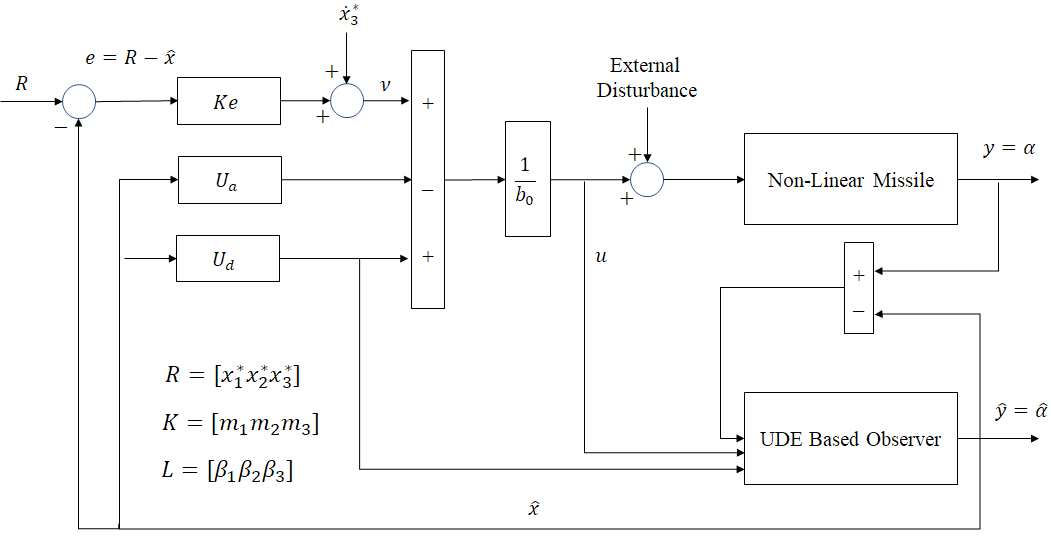
\includegraphics[width=0.8\linewidth]{block_diag}
		\end{figure}

\end{frame}


%------------------------------------------------
%SUBSECTION1
\subsection{Controller Design} % A subsection can be created just before a set of slides with a common theme to further break down your presentation into chunks
\begin{frame}
	\frametitle{Input Output Linearization}
	\textbf{Implementation of IOL to cancel non-linearities of missile model} 
	\begin{itemize}
		\item To make relative degree = order of equation, $d_n \approx 0$
		\item Within $-20^\circ\le \alpha \le20^\circ$, $\cos(\alpha) \approx 1$
		\item Now obtaining $\dddot{\alpha}$ gives
	\end{itemize}

\begin{eqnarray*}
\begin{aligned}
	\dddot{\alpha}&=K_q M^2(3a_m\alpha^2+2b_m|\alpha|+c_m\Big(-7+\frac{8M}{3}\Big))\dot{\alpha}\\ 
	&\quad - K_q M^2d_m\omega_a\delta+K_{\alpha}M(6a_n\alpha+2b_n sgn(\alpha))\dot{\alpha}^2\\ 
	&\quad + K_\alpha M(3a_n\alpha^2+2b_n|\alpha|+c_n\Big(2-\frac{M}{3}\Big))\ddot{\alpha}\\ 
	&\quad + K_q M^2d_m\omega_a\delta_c \label{a3dot}
\end{aligned}
\label{eq4}
\end{eqnarray*}

\end{frame}

\begin{frame}
\frametitle{Input Output Linearization}
When represented in IOL form $\dddot{\alpha} = a + b\delta_c$ we get; 
\begin{eqnarray*}
	\begin{aligned}
		a &= K_qM^2(3a_m\alpha^2+2b_m|\alpha|+c_m\Big(-7+\frac{8M}{3}\Big))\dot{\alpha} \\ 
		&\quad -K_qM^2d_m\omega_a\delta+K_\alpha M(6a_n\alpha+2b_nsgn(\alpha))\dot{\alpha}^2\\ 
		&\quad+K_\alpha M(3a_n\alpha^2+2b_n|\alpha|+c_n\Big(2-\frac{M}{3}\Big))\ddot{\alpha} \\
		b &= K_q M^2d_m\omega_a \nonumber
	\end{aligned}
	\label{eq5}
\end{eqnarray*}

Thus the control law is, 

\begin{eqnarray*}
	\begin{aligned}
%		without this comment the equations on this slide disappear. No idea why.
		\delta_c &= \frac{1}{b}(u_a+\nu) \\ \label{iol_control}
		u_a &= -a \label{ua_eqn}\\
		\nu &= \dddot{\alpha}^\ast+m_1(\alpha^\ast-\alpha) + m_2(\dot{\alpha}^\ast-\dot{\alpha}) + m_3(\ddot{\alpha}^\ast-\ddot{\alpha}) \label{nu_eqn}
	\end{aligned}
	\label{eq5}
\end{eqnarray*}

\end{frame}
%-------------------------------------------------------------------------------------------------------------------------------------------
\begin{frame}
\frametitle{UDE Augmented IOL Controller}
\textbf{The UDE control law utilizes a new term $u_d$ as follows;}
\begin{itemize}  % Shows text in bullet point 		
		\item $\delta_c = \frac{1}{b}\Big[u_a+u_d+\nu\Big]$ where, $u_d = -\hat{d}$
		\item $\hat{d}$ is an estimate of the lumped disturbance and uncertainties $d$;
%\end{itemize}

%\textbf{$\hat{d}$ is an estimate of the lumped disturbance and uncertainties $d$;}
%\begin{itemize}
		\begin{enumerate}
			\item $\dddot{\alpha} = a + b\delta_c + d$
			\item $d = \Delta a + \Delta b \delta_c + w$
			\item $\hat{d}=G_f(s)d$
			\item $G_f(s)=\frac{1}{1+s\tau}$ \\
		\end{enumerate}
\end{itemize}

\begin{itemize}
	\item Thus, we finally get
	$u_d=\frac{-1}{\tau}\Big[\ddot{\alpha}-\int{\nu dt}\Big] \label{ude}$
	
\end{itemize}

\end{frame}
%%------------------------------------------------------------------------------------------------------------------------------------------
\begin{frame}
\frametitle{UDE Observer based Control law}
	\textbf{A Luenberger like UDE Observer has been designed \textcolor{red}{CITE EVERYWHERE}}


\begin{itemize}  % Shows text in bullet point 		
	\item $\dddot{\alpha}$ is separated into linear and non-linear ($d_1$) terms; $\dddot{\alpha} = a_1 \alpha + a_2 \dot{\alpha} + a_3 \ddot{\alpha} + d_1 + b\delta_c$
	
	\item Then the non-linear term $d_1$ and uncertainties are clubbed into a lumped term $d_2$, such that; \\
	$\dddot{\alpha} = a_{1o} \alpha + a_{2o} \dot{\alpha} + a_{3o} \ddot{\alpha} + b_o\delta_c + d_2$\\
	
	\item This expressed in state space form can then be used to design the observer:
	\begin{eqnarray*}
		\begin{aligned}
			\dot{x}_1 &= x_2 \\
			\dot{x}_2 &= x_3 \\
			\dot{x}_3 &= a_{1o}x_1 + a_{2o}x_2 + a_{3o}x_3 + b_o \delta_c + d_2 \\
			y &= x_1 \label{rx1}
		\end{aligned}
		\label{eq5}
	\end{eqnarray*}
	
\end{itemize}

\end{frame}

\begin{frame}
\frametitle{UDE Observer based Control law}

Now since the equations are represented in a linear manner, a Luenburger like UDE Observer is designed by introducing the observer poles $[\beta_1 \beta_2 \beta_3]$
\begin{eqnarray*}
	\begin{aligned}
		\dot{\hat{x}}_1 &= \hat{x}_2 + \beta_1 e_o\\
		\dot{\hat{x}}_2 &= \hat{x}_3 + \beta_2 e_o\\
		\dot{\hat{x}}_3 &= a_{1o}\hat{x}_1 + a_{2o}\hat{x}_2 + a_{3o}\hat{x}_3 + b \delta_c + \hat{d}_2 + \beta_3 e_o\\		
		\hat{y} &= \hat{x}_1 \label{ss1}
	\end{aligned}
	\label{eq5}
\end{eqnarray*}

Here, the term $d_2$ representing the non-linearities and uncertainties is estimated by UDE

\end{frame}



\begin{frame}
\frametitle{Stability Analysis}

\begin{eqnarray}
\begin{aligned}
\begin{bmatrix}
\dot{e}_c \\
\dot{e}_o \\
\dot{\tilde{d}}_2
\end{bmatrix} =& 
\begin{bmatrix}
(A - BK) & -(BK) & -B_d \\
0 & (A - LC) & B_d \\
0 & 0 & -\frac{1}{\tau}
\end{bmatrix}
\begin{bmatrix}
e_c \\
e_o \\
\tilde{d}_2
\end{bmatrix}	
& + 
\begin{bmatrix}
0 \\
0 \\
1
\end{bmatrix} \dot{d}_2 \label{sr8}
\end{aligned}
\end{eqnarray}

\begin{eqnarray}
\begin{vmatrix}
sI - (A - BK)
\end{vmatrix}
\begin{vmatrix}
sI - (A - LC)
\end{vmatrix}
\begin{vmatrix}
s - (-\frac{1}{\tau})
\end{vmatrix} = 0 \label{sr9}
\end{eqnarray}

\begin{itemize}
	\item $(A, B)$ is controllable and $(A, C)$ is observable
	\item $\tau$ is strictly a positive number
	\item Selecting appropriate controller and observer poles ensures stability of error dynamics
	\item Also if $\dot{d}_2 \ne 0$, then bounded-input, bounded-output stability can be assured. 
\end{itemize}


\end{frame}


%%--------------------------------------------- --
%% Start of fifth slide
%%------------------------------------------------------------------------------------------------------------------------------------------

\begin{frame}
\frametitle{Simulations}
\textbf{Parameters for simulation}
\begin{itemize}  % Shows text in bullet point 		
		\item Reference signal: \\  
		\begin{equation}
			\alpha^{*}=
			\begin{cases}
			15^{\circ}, & \text{if $0 \leq t \leq2 ~ s$}\\
			-8^{\circ}, & \text{if $2 < t \leq4 ~ s$}\\
			10^{\circ}, & \text{if $4 < t \leq6 ~ s$} \label{ref_sig}\\ 
			\end{cases} \nonumber
		\end{equation}
		\item Tracking Constraints:
		\begin{enumerate}
			\item To be tracked with a time constant of less than $0.25s$
			\item Less than 10\% overshoot
			\item Less than 1\% steady-state error
		\end{enumerate}
		\item Pole placement to meet this target:
		\begin{enumerate}
			\item Controller gains $[m_1\ m_2 \ m_3]$ placed at $s_{1,2,3} = -12$
			\item Observer gains $[\beta_1 \ \beta_2 \ \beta_3]^T$ placed at $s_{1,2,3} = -360$
		\end{enumerate}
	
		\item Controller and observer designed at M = 2.25 (mid-point of Mach envelope)
	\end{itemize}

\end{frame}

%%-----------------------------------------------------------------------------------------------------------------------------------------
\begin{frame}
\frametitle{Case I: UDE with Mach Dynamics \& External Disturbance}

\begin{itemize}
	\item UDE simulated with varying mach and external disturbance
	\item Mach i.c is $M(0) = 2.5$ and follows $M$ equation \textcolor{red}{reference??} till $M = 2$
	\item Extrenal disturbance modeled as sinusoidal amplitude $8^\circ$ and frequency $0.25 Hz$
\end{itemize}

\begin{figure}
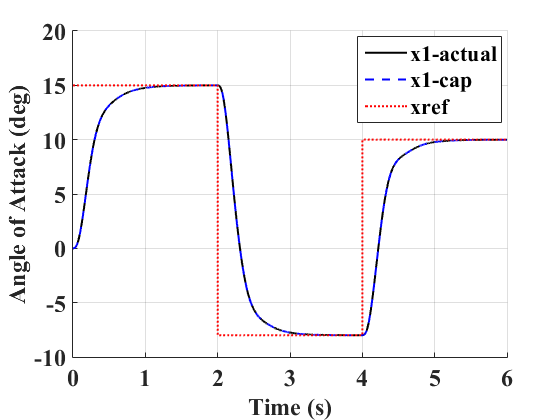
\includegraphics[width=4cm]{1_ude_varying-mach_x1}
%\title{Output response}
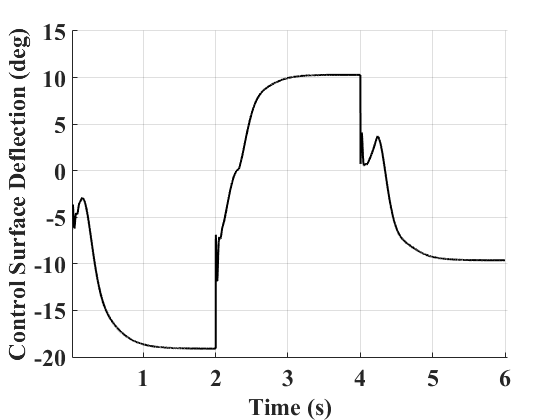
\includegraphics[width=4cm]{2_ude_varying-mach_control}
\end{figure}


\end{frame}	

\begin{frame}
\frametitle{Case I: UDE with Mach Dynamics \& External Disturbance}
\begin{figure}
	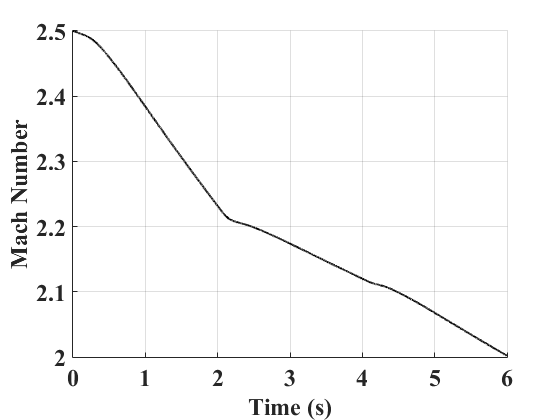
\includegraphics[width=4cm]{3_ude_varying-mach_mach}
	%\title{Output response}
	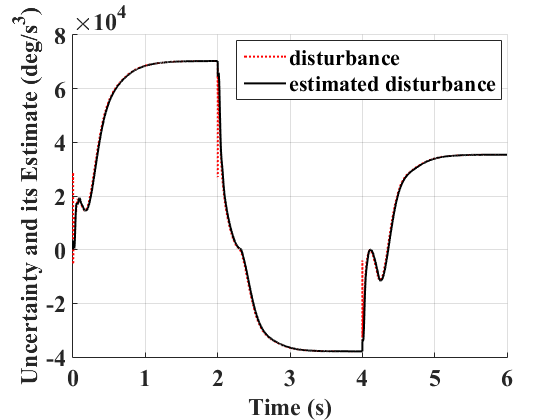
\includegraphics[width=4cm]{4_ude_varying-mach_dist}
\end{figure}
	\begin{center}
	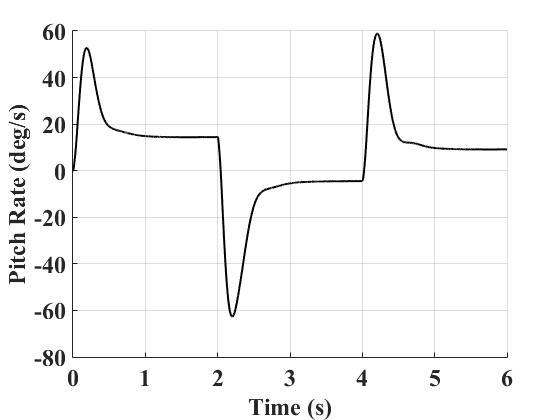
\includegraphics[width=4cm]{5_ude_varying-mach_pitch}
	\end{center}
\end{frame}


\begin{frame}
\frametitle{Case II: Comparative Study With Aerodynamic Uncertainties}
\begin{itemize}  % Shows text in bullet point 		
		\item Comparative analysis of UDE has been done against Predictive Control (PC) and Sliding Mode Control (SMC) \textcolor{red}{ADD Citation}
		\item Uncertainty of $+30\%$ in aerodynamic force coefficient $C_n$ and $-30\%$ in aerodynamic moment coefficient $C_m$
		\item Mach has been maintained at the nominal constant of $M = 2.25$ 
		\item No external disturbances added to the system.
\end{itemize}
\end{frame}
%-------------------------------------------------------------------------------Figure 4-------------------------------------------------------------------
%
\begin{frame} 
\frametitle{Case II: Comparative Study With Aerodynamic Uncertainties}
\begin{figure}
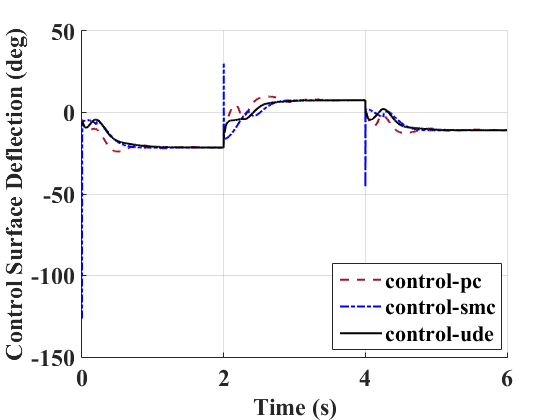
\includegraphics[width=4cm]{control_kcn_13_kcm_07}
%\title{Output response}
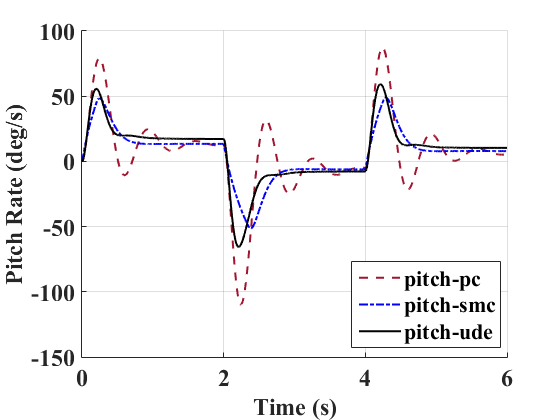
\includegraphics[width=4cm]{pitch_kcn_13_kcm_07}
%\caption{Output response}
%\end{figure}
\begin{center}
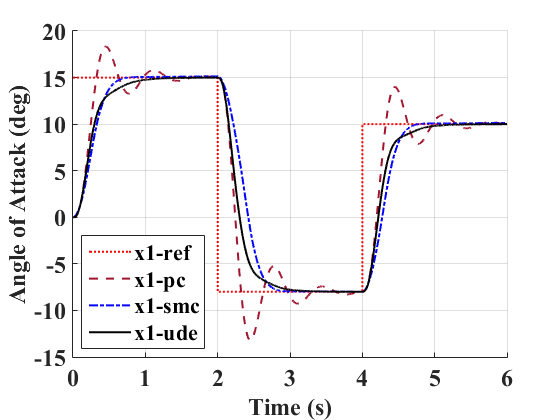
\includegraphics[width=4cm]{x1_kcn_13_kcm_07}
\end{center}
\end{figure}
\end{frame}

\begin{frame}
	\frametitle{Results and conclusions}
	\begin{itemize}
		\item Results of CASE I
		\begin{enumerate}
			\item Tracking performance is as desired and control effort stays smooth and within the practical bounds of  $\pm30^\circ$
			\item UDE observer is able to estimate states quickly and accurately
			\item Estimation of disturbance by UDE is minimally delayed and follows closely to the actual value
		\end{enumerate}
		
		\item Results of CASE II
		\begin{enumerate}
			\item Due to aerodynamic uncertainty, PC has overshoots in tracking. UDE and SMC are smooth 
			\item Control effort of PC is oscillatory. SMC has high overshoots at transition points. UDE is able to provide smooth control within $\pm 30^\circ$
			\item Pitch graph of PC is oscillatory while SMC is slightly delayed. Pitch graph of UDE is on point.
		\end{enumerate}
	\end{itemize}	
	
\end{frame}

\begin{frame}
	\frametitle{Novelty}
	\begin{itemize}
		\item Despite uncertainties such as varying mach (case I) and varying aerodynamic constants (case II) and even the presence of external disturbance (case I), UDE is able to provide robust tracking control.
		\bigskip
		
		\item Only the frequency bound (captured through $\tau$) of the external disturbance and uncertainty is required to provide robust tracking with UDE. There is no dependency on the magnitude bounds of the disturbance/uncertainty. \textcolor{red}{include in UDE slide also...relate to $\tau$}
		\bigskip
		
		\item Unlike PC and SMC simulations which have used the actual states while implementing the control law, UDE simulation has utilized the estimated
		states obtained from the UDE observer. As is well known, use of estimated states might result in degraded performance; in contrast the proposed strategy utilizes the estimated states and still proves its worthiness.
\end{itemize}
\end{frame}


\begin{frame}
\frametitle{Future Work}
\begin{itemize}

	\item Design of an integrated pith-yaw-roll autopilot 
	\bigskip
	\item Application of UDE to a nonlinear missile model with and without prior linearization of the model
	
\end{itemize}
\end{frame}


\begin{frame}
	\frametitle{References}
\end{frame}
%---------------------------------------------------------------------------------------------------------------------------------


	\begin{thebibliography}{1}



%\bibitem{IEEEhowto:kopka}
%H.~Kopka and P.~W. Daly, \emph{A Guide to \LaTeX}, 3rd~ed.\hskip 1em plus
  %0.5em minus 0.4em\relax Harlow, England: Addison-Wesley, 1999.
	%
%% Reference 1
%\bibitem{song2002}
%Chanho Sung, and Yoon-Sik Kim, \lq \lq A new approach to motion modeling and autopilot design of skid-to-turn missile," Trans. on Control, Automation, and System Engg, 4(3), Sep 2002, pp. 231-238. 
%
%% Reference 2
%\bibitem{kang2009}
%S. Kang, and H. J. Kim, \lq \lq Roll-pitch-yaw integrated robust autopilot design for a high angle-of-attack missile," J. of Guidance, Control, and Dynamics, Sep-Oct 2009, pp. 1622-1628.
%
%%Reference 3
%\bibitem{sirisha2012}
%C. V. Sirisha, Ranajit Das, and R. N. Bhattacharjee, \lq \lq Disturbance estimation based roll autopilot design for tactical missiles," Proc. Advances in Control and Optimization of Dynamic Systems, ACDOS - 2012, pp. 1-5.

%%Reference 4
%\bibitem{luo2015}
%D. Luo, and Y. Liu, \lq \lq Roll autopilot using variable structure control based on new reaching law," Int. J. of Technical Research and Application, 23, July 2015, pp. 29-32.
%
%%Reference 5
%\bibitem{chen2016}
%W. H. Chen, J. Yang, and Z. Zhao, \lq \lq Robust control of uncertain nonlinear systems: a nonlinear DOBC approach," ASME J. of Dynamic Systems, Measurement and Control, vol.138, Jul 2016, in press.
%
%%Reference 6
%\bibitem{mohammadi2016}
%M. R. Mohammadi, M. F. Jegarhandi, and A. Moarrefianpour, \lq \lq Robust roll autopilot design couplings of a tactical missile," Aerospace Science and Tech., 51, 2016, pp. 142-150.
%
%%Reference 7
%\bibitem{nesline1984}
%F. W. Nesline, and P. Zarchan, \lq \lq Why modern controllers can go unstable in practice,"' J. Guidance, Control and Dynamics, 7(4), Jul-Aug 1984, pp. 495-500.
%
%%Reference 8
%\bibitem{chwa2004}
%D. Chwa, J. Y. Choi, and J. H. Seo, \lq \lq Compensation of actuator dynamics in nonlinear missile control," IEEE Trans. Control Systems Technology, 12(4), July 2004, pp. 620-626.
%
%%Reference 9
%\bibitem{parkhi2010}
%P. Parkhi, B. Bandyopadhyay, and M. Jha, \lq \lq Design of roll autopilot for a tail controlled missile using sliding mode technique," Proc. Int. workshop on Variable Structure Systems, Mexico, June 2010, pp. 389-394.
%
%%Reference 10
%\bibitem{gezer2014}
%R. B. Gezer, and A. K. Kutay, \lq \lq Robust model following control design for missile roll autopilot," Proc. UKACC Int. Conf. on Control, Loughborough,  U. K., July 2014, pp. 7-12.

%Reference 11
\bibitem{talole2011}
S. E. Talole, A. A. Godbole, and J. P. Kolhe, \lq \lq Robust autopilot design for tactical missiles," J. of Guidance, Control and Dynamics, 34(1), Jan - Feb 2011, pp. 107-117.
%
%%Reference 12
%\bibitem{sankar2016}
%R. B. Sankar, B. Bandyopadhyay, and H. Arya, \lq \lq Design of roll autopilot for a tail controlled missile using sliding mode technique," Proc. Int. Workshop on Variable Structure Systems, Mexico, June 2010, pp. 389-394.

%Reference 13
\bibitem{zhong2004}
Q. C. Zhong, and D. Rees, \lq \lq Control of LTI systems based on an uncertainty and disturbance estimator," ASME Trans. J. of Dynamic systems, Measurement and Control, 126(4), 2004, pp. 905-910.

%Reference 14
\bibitem{ogata2010}
K. Ogata, Modern Control Engineering, 5th ed. PHI, New Delhi, 2010, pp. 743-746.

%%Reference 13
%\bibitem{zhong2004}
%Q. C. Zhong, and D. Rees, \lq \lq Control of LTI systems based on an uncertainty and disturbance estimator," ASME Trans. J. of Dynamic systems, Measurement and Control, 126(4), 2004, pp. 905-910.


\end{thebibliography}
%--------------------------------------------------------------------------
\subsection*{Thank You} % A subsection can be created just before a set of slides with a common theme to further break down your presentation into chunks
\begin{frame}
%\hskip4cm
\textbf{\LARGE Thank You!} \\[20pt]
%\hskip3cm
\end{frame}

\end{document} 
